% =========================================================
% INTRODUCCIÓN
% =========================================================
\chapter{Introducción}
\label{cap:introduccion}

\section{Formación Planetaria y Acreción de Pebbles}

La formación planetaria constituye uno de los problemas fundamentales de la astrofísica moderna. Actualmente se acepta que los planetas se forman en discos protoplanetarios compuestos por gas y polvo que rodean a estrellas jóvenes durante las primeras etapas de su evolución. En estos discos, partículas microscópicas de polvo colisionan y crecen progresivamente hasta formar cuerpos de mayor tamaño, eventualmente dando origen a planetesimales y planetas.

Sin embargo, comprender cómo ocurre este proceso de crecimiento continúa siendo un desafío teórico importante. Los modelos clásicos de acreción enfrentan diversas dificultades, particularmente en las etapas intermedias de crecimiento, donde partículas de tamaño centimétrico a métrico experimentan una rápida deriva radial hacia la estrella central antes de poder formar cuerpos planetarios masivos. Este problema, conocido como la ``drift barrier'', limita significativamente la eficiencia de los modelos tradicionales de formación planetaria \citep{Laibe2012, Blum2018}.

En las últimas décadas, el paradigma de \textit{pebble accretion} ha emergido como una posible solución a estas dificultades. En este escenario, pequeños sólidos aerodinámicamente acoplados al gas ---denominados \textit{pebbles}--- pueden ser acrecidos de manera altamente eficiente por embriones planetarios, acelerando considerablemente el crecimiento de planetas \citep{Lambrechts2014, Bitsch2015, 2019ApJ...883..192A}. Este mecanismo no solo permite explicar escalas temporales compatibles con la vida útil observada de los discos protoplanetarios, sino también reproduce diversas propiedades observadas en sistemas planetarios extrasolares \citep{Johansen2017, Ormel2017, Drazkowska2023, Lyra2023}.


\section{El Problema de los Discos Suaves}

Los modelos modernos de evolución de discos protoplanetarios permiten estudiar cómo evoluciona el flujo de sólidos a lo largo del tiempo y cómo este depende de las propiedades físicas del disco. Frameworks como \textit{Pebble Predictor} \citep{Drazkowska2021} modelan la evolución del gas y del polvo, permitiendo calcular el flujo radial de pebbles hacia distintas regiones del disco protoplanetario. Asimismo, herramientas más recientes como \textit{TripodPy} \citep{Pfeil2024_teoria, Pfeil2025_codigo} permiten incorporar modelos avanzados de evolución de polvo y distribuciones de tamaño multipoblacionales.

Estos resultados pueden posteriormente utilizarse como input para modelos de \textit{pebble accretion} o esquemas de postprocesado orientados a estudiar el crecimiento de embriones planetarios y la evolución composicional de sistemas planetarios.

Sin embargo, muchos de estos modelos asumen discos protoplanetarios suaves (\textit{smooth disks}), es decir, discos con perfiles radiales continuos y sin subestructuras locales. Esta aproximación presenta limitaciones importantes desde el punto de vista físico.

En discos suaves, los pebbles experimentan una rápida deriva radial producto del acoplamiento aerodinámico con el gas. Debido a que el gas orbita a velocidades ligeramente sub-Keplerianas, las partículas sólidas sienten un \textit{headwind} que les hace perder momento angular y migrar hacia la estrella central. En ausencia de trampas de presión o estructuras capaces de modificar localmente el gradiente de presión, este proceso produce un transporte eficiente y continuo de sólidos hacia las regiones internas del disco.

Como consecuencia, los modelos \textit{smooth} pueden sobreestimar el flujo de pebbles disponible para acreción planetaria en el disco interno, afectando significativamente las predicciones sobre crecimiento planetario y eficiencia de acreción \citep{Lau2024, Appelgren2020, Appelgren2025}.

En este contexto, incorporar subestructuras en modelos de evolución de discos resulta fundamental para construir escenarios más realistas de formación planetaria. Las perturbaciones locales del perfil de presión pueden modificar significativamente el transporte de sólidos y regular el flujo de pebbles a través del disco.


\section{Subestructuras en Discos Protoplanetarios}

Observaciones de alta resolución realizadas durante la última década han revolucionado nuestra comprensión de los discos protoplanetarios. En particular, el observatorio ALMA (\textit{Atacama Large Millimeter/submillimeter Array}) ha revelado que numerosos discos presentan complejas subestructuras radiales, incluyendo anillos, gaps, cavidades y regiones localizadas de acumulación de polvo \citep{ALMAPartnership2015, Andrews2018}.

Uno de los ejemplos más emblemáticos corresponde al disco protoplanetario de HL Tauri, cuyas observaciones mostraron por primera vez una serie de anillos y gaps bien definidos incluso en etapas tempranas de evolución del disco \citep{ALMAPartnership2015}. Posteriormente, múltiples estudios confirmaron que este tipo de estructuras son comunes en discos protoplanetarios observados a longitudes de onda milimétricas \citep{Andrews2018}.


\begin{figure}[ht]
    \centering
    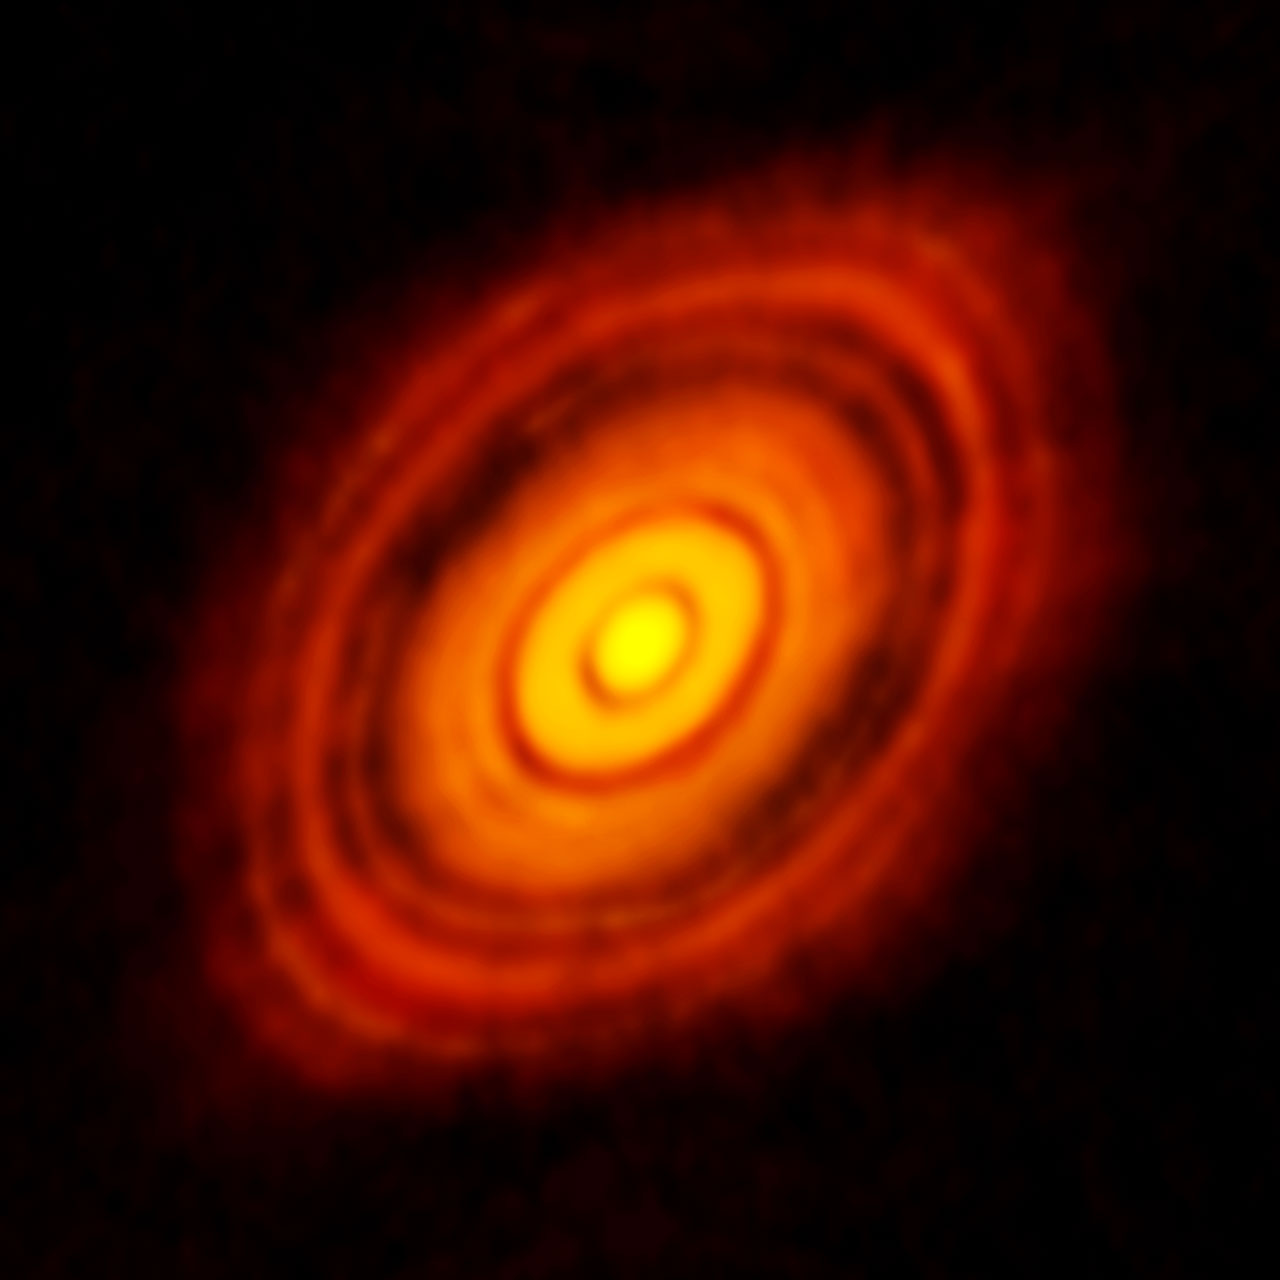
\includegraphics[width=0.8\textwidth]{figures/HL tauri.jpg}
    \caption{Disco protoplanetario alrededor de HL Tauri observado con ALMA. La imagen revela estructuras anulares y regiones oscuras asociadas con posibles procesos de formación planetaria. Creditos: ALMA (ESO/NAOJ/NRAO).}
    \label{fig:HLTau}
\end{figure}


Diversos mecanismos físicos han sido propuestos para explicar el origen de estas subestructuras. Entre ellos se incluyen la interacción disco-planeta, inestabilidades magnetohidrodinámicas, variaciones locales de viscosidad asociadas a \textit{dead zones}, transiciones químicas cercanas a \textit{snowlines} y procesos hidrodinámicos capaces de modificar localmente el perfil de presión del gas \citep{Akiyama2016, Andrews2018, Kanagawa2016}.

Desde el punto de vista dinámico, estas estructuras pueden actuar como trampas de presión (\textit{pressure bumps}) capaces de alterar significativamente el transporte radial de sólidos. En regiones donde el gradiente de presión cambia de signo o disminuye localmente, la deriva radial de pebbles puede ralentizarse o incluso detenerse temporalmente, favoreciendo la acumulación de polvo y reduciendo el flujo de material sólido hacia el interior del disco \citep{Pinilla2012, Pierens2024, Baruteau2019}.

Como consecuencia, las subestructuras no solo modifican la distribución espacial de sólidos, sino también las condiciones bajo las cuales ocurre \textit{pebble accretion} \citep{Andama2022, Ataiee2018}. Esto puede impactar directamente las escalas temporales de crecimiento planetario, la eficiencia de acreción y la composición final de los planetas formados.


\section{Pebble Flux y Composición Planetaria}

El flujo radial de pebbles constituye uno de los parámetros más importantes en modelos modernos de formación planetaria. La cantidad de material sólido transportado a través del disco determina directamente la masa disponible para acreción planetaria y, por lo tanto, controla las escalas temporales y la eficiencia del crecimiento de embriones planetarios.

Además de regular el crecimiento, el \textit{pebble flux} también juega un rol fundamental en la composición final de los planetas. A medida que los pebbles migran radialmente a través del disco, atraviesan distintas regiones térmicas donde materiales volátiles pueden condensarse o sublimarse. En particular, la \textit{snowline} del agua representa una transición crítica para la distribución composicional de sólidos en discos protoplanetarios.

La evolución temporal de estas regiones puede modificar significativamente la composición de los pebbles disponibles para acreción \citep{Booth2017, Booth2019}. Como consecuencia, cambios en el transporte radial de sólidos pueden producir variaciones importantes en el contenido de agua y volátiles de los planetas formados \citep{Banzatti2023}.

En este contexto, diversos trabajos han propuesto que mecanismos capaces de regular el flujo de pebbles podrían favorecer la formación de planetas ricos en agua, comúnmente denominados \textit{waterworlds} \citep{McCloat2025, Krijt2025, Bitsch2021, Astrakhantsev2026}. Comprender cómo las subestructuras afectan el transporte de sólidos resulta, por tanto, fundamental para estudiar la conexión entre dinámica de discos protoplanetarios y composición planetaria.


\section{Transporte Tardío de Agua y Rol de las Subestructuras}

Aunque diversos estudios han mostrado que el transporte radial de pebbles puede desempeñar un papel importante en la composición de los planetas formados, la mayoría de estos escenarios asumen un suministro relativamente continuo de material sólido hacia las regiones internas del disco \citep{Appelgren2020, Lau2024}.

Sin embargo, la presencia de subestructuras observadas en discos protoplanetarios introduce la posibilidad de que el flujo de pebbles sea modulado temporalmente \citep{Pinilla2012, Stammler2022}. En particular, la retención de polvo en reservorios asociados a gaps podría retrasar la llegada de material rico en volátiles hasta etapas más avanzadas de evolución del disco, cuando la \textit{snowline} del agua se encuentra más cerca de la región terrestre \citep{Oka2011, Bitsch2015}.

Esto plantea la posibilidad de que la interacción entre la evolución de la \textit{snowline} y la liberación de estos reservorios tenga consecuencias importantes sobre la entrega tardía de agua y la composición final de los planetas \citep{Banzatti2023, McCloat2025}.


\subsection{Hipótesis de Trabajo}

En este trabajo se propone que la retención temporal de pebbles producida por subestructuras de origen planetario puede retrasar la llegada de material rico en volátiles hacia las regiones internas del disco. Si la \textit{snowline} atraviesa estos reservorios antes de que sean completamente liberados, el cambio en las propiedades de fragmentación del polvo puede desencadenar una liberación tardía de pebbles, fenómeno conocido como \textit{pebble snow} \citep{Drazkowska2021, McCloat2025}.

Se plantea que este mecanismo puede modificar significativamente el flujo de sólidos disponible para acreción planetaria y favorecer el transporte tardío de agua hacia regiones cercanas a la zona habitable, afectando tanto el crecimiento como la composición final de los planetas formados \citep{Bitsch2021, Krijt2025, Astrakhantsev2026}.

\section{Objetivos del Trabajo}

Con el objetivo de evaluar esta hipótesis, se desarrolló un framework computacional basado en TripodPy capaz de modelar discos protoplanetarios estructurados mediante perturbaciones locales del perfil de presión del gas.

A partir de estas simulaciones, se analizó cómo distintas configuraciones de gaps y \textit{pressure bumps} afectan el transporte radial de sólidos y la evolución temporal del \textit{pebble flux}.

Adicionalmente, se desarrolló un esquema de postprocesado orientado a estudiar acreción de pebbles y evolución composicional, incorporando efectos asociados a la migración de la \textit{snowline} y al transporte diferencial de materiales volátiles.

Finalmente, este trabajo busca explorar si la regulación del flujo de pebbles producida por subestructuras puede favorecer escenarios de formación de planetas ricos en agua y modificar las predicciones tradicionales de modelos basados en discos suaves.
